\section{Energía, transporte y litio}

En la actualidad se utilizan distintas formas para generar energía y pueden 
dividirse en dos grandes tipos, las renovables y las no-renovables. Estas últimas
dominan la producción de energía mundial y están compuestas principalmente por 
combustibles fósiles y centrales nucleares, mientras que las energías renovables
abarcan más variantes como la biomasa, la hidráulica, la eólica y la solar, pero 
aún no son lo suficientemente utilizadas. Una de las particularidades de estas 
fuentes de energías renovables es su producción intermitente mientras que el 
consumo de la misma, independientemente de cómo se genere, es a demanda. Esto 
hace que sea necesario la involucración de vectores energéticos que permitan 
almacenar y transportar el excedente de energía que se genera en sus períodos de 
mayor producción.

El sector del transporte por tierra, maritimo y áereo es responsable de más de un 
tercio de las emisiones de CO$_2$ debido a su dependencia en los combustibles 
fósiles. Dicho esto se debe fomentar opciones de desplazamiento menos intensivas
en carbono y con tecnologías más eficientes, como los vehículos eléctricos (EV).
Los EV poseen una eficiencia en su motor que ronda el 80\%, comparese este valor 
con la eficiencia del 30\% de los motores a combustión eléctrica, y tienen un 
funcionamiento silencioso. En los últimos años se ha producido un crecimiento 
exponencial en las ventas anuales de los mismos, como puede observarse en la
Figura \ref{fig:ev-volumes}. En la última década, dichas ventas aumentaron 
aproximadamente un 500\% y se estima que para la próxima década las ventas se 
multipliquen por 10. Estas ventas están concentradas en China y en algunos países
y estados de Europa y Estados Unidos, respectivamente, debido a que en los países
en desarrollo y emergentes influye negativamente su costo alto de adquisición y 
una falta de infraestructura para la recarga de sus baterías.
\begin{figure}[h!]
    \centering
    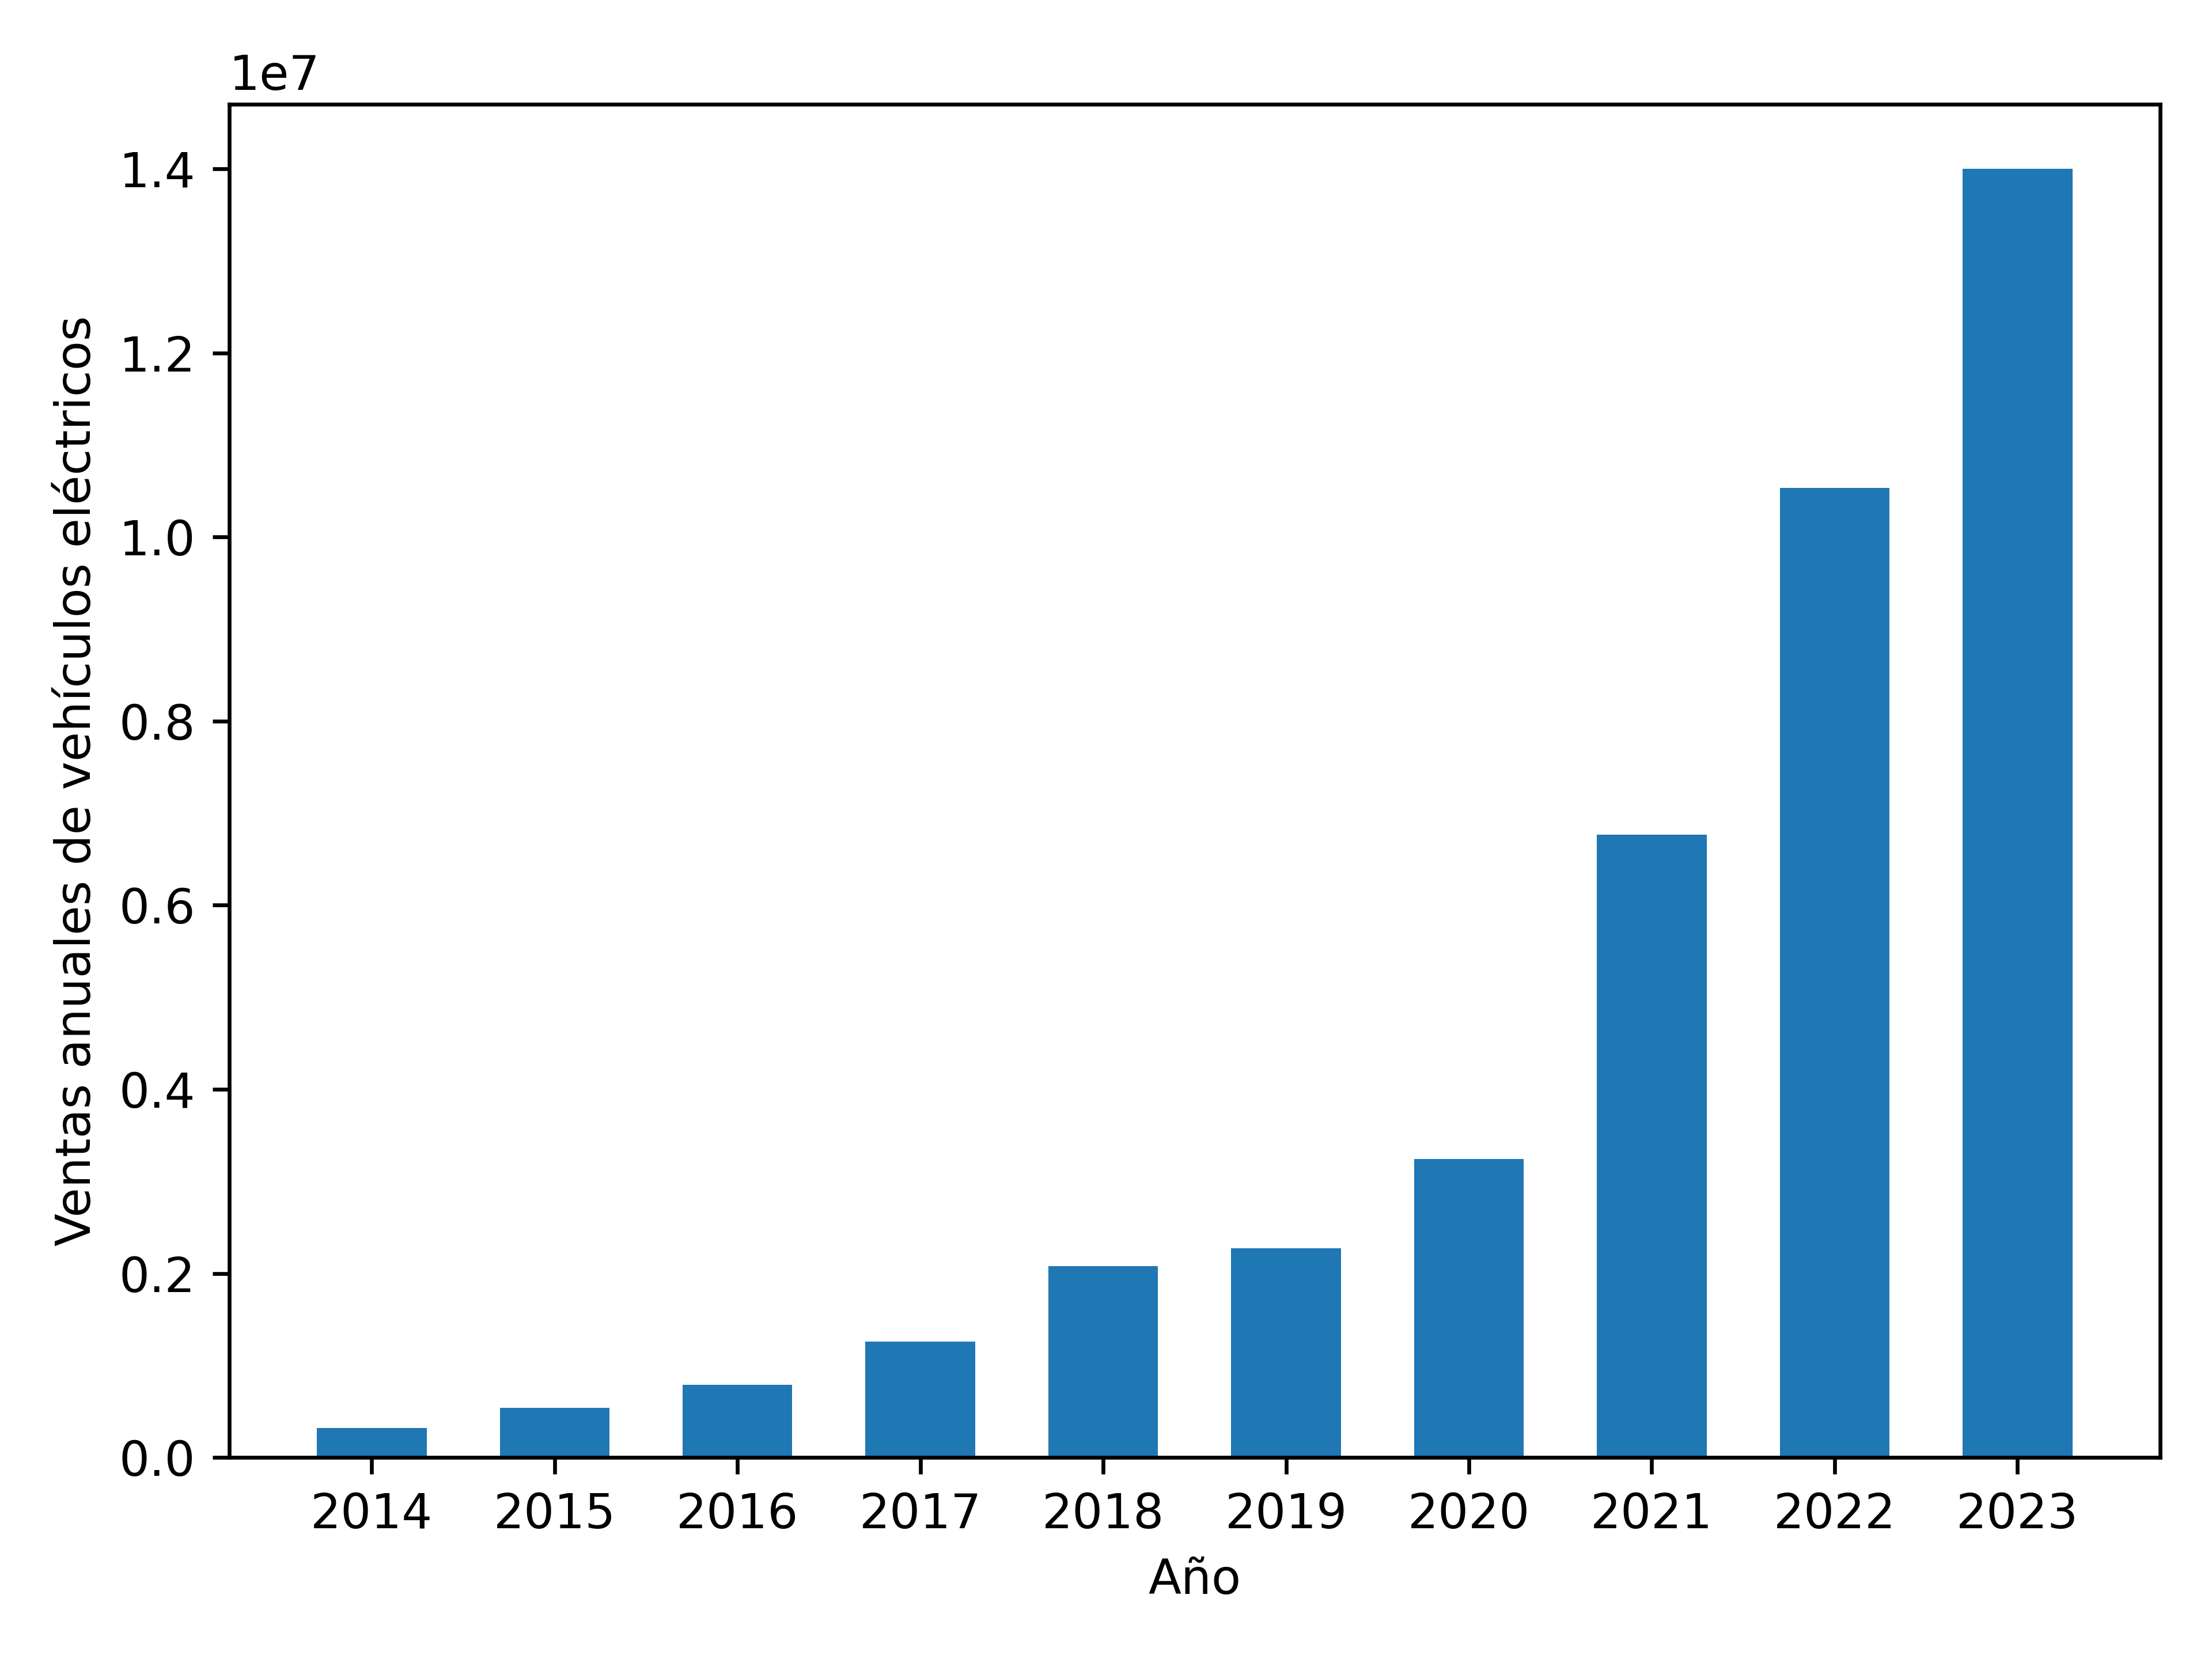
\includegraphics[width=.8\textwidth]{Introduccion/energia/ev-volumes.png}
    \caption{Ventas anuales de vehículos eléctricos en la última década. Se 
    proyecta que para el 2030 las ventas asciendan a las 40 millones de unidades 
    frente a las 3 millones del año 2020. Fuente: \cite{EVV}.}
    \label{fig:ev-volumes}
\end{figure}

El sector energético en Argentina depende altamente de la utilización de 
combustibles fósiles, donde la generación de energía está dominada por el gas 
natural (65\%) y le siguen las centrales hidroeléctricas (18\%), plantas nucleares
(8\%), parques eólicos (7\%) y solares (1\%). En cuanto al potencial de 
producción de fuentes renovables, Argentina tiene una gran capacidad en sus 
fuentes eólicas y solares por desarrollar. Además, es el cuarto productor más 
grande de litio, que es un mineral crítico para la manufactura de sistemas de 
almacenamiento y transporte de energía, claves para la transición energética. 
Otros metales y minerales críticos son grafito, cobre, níquel, manganeso, cobalto 
y silicio; entre ellos, el litio representa el 7\% de la demanda para vehículos 
eléctricos mientras que para almacenamiento en la red el porcentaje es del 10\%.

En la Figura \ref{fig:iea-Li} se muestra la proyección en la demanda total de 
litio por año y aplicación, donde la mayor contribución se encuentra para la 
utilización del mismo en vehículos eléctricos mientras que una menor contribución 
se espera en aplicaciones de sistemas de almacenamiento estacionarios y otras 
aplicaciones que incluyen dispositivos electrónicos, medicamentos, lubricantes, 
entre otras \cite{IEA}. Pueden diferenciarse dos regiones en el histograma, la 
primera de ellas entre el año 2022 y el 2035, donde los aumentos porcentuales de 
la demanda de litio con respecto a 5 años atrás son del 74\%, 99\% y 76\%. Luego
del año 2035 al 2040 el cambio se encuentra en el 32\% y continúa disminuyendo 
al 10\% y al 3\% en los años subsiguientes.
\begin{figure}[h!]
    \centering
    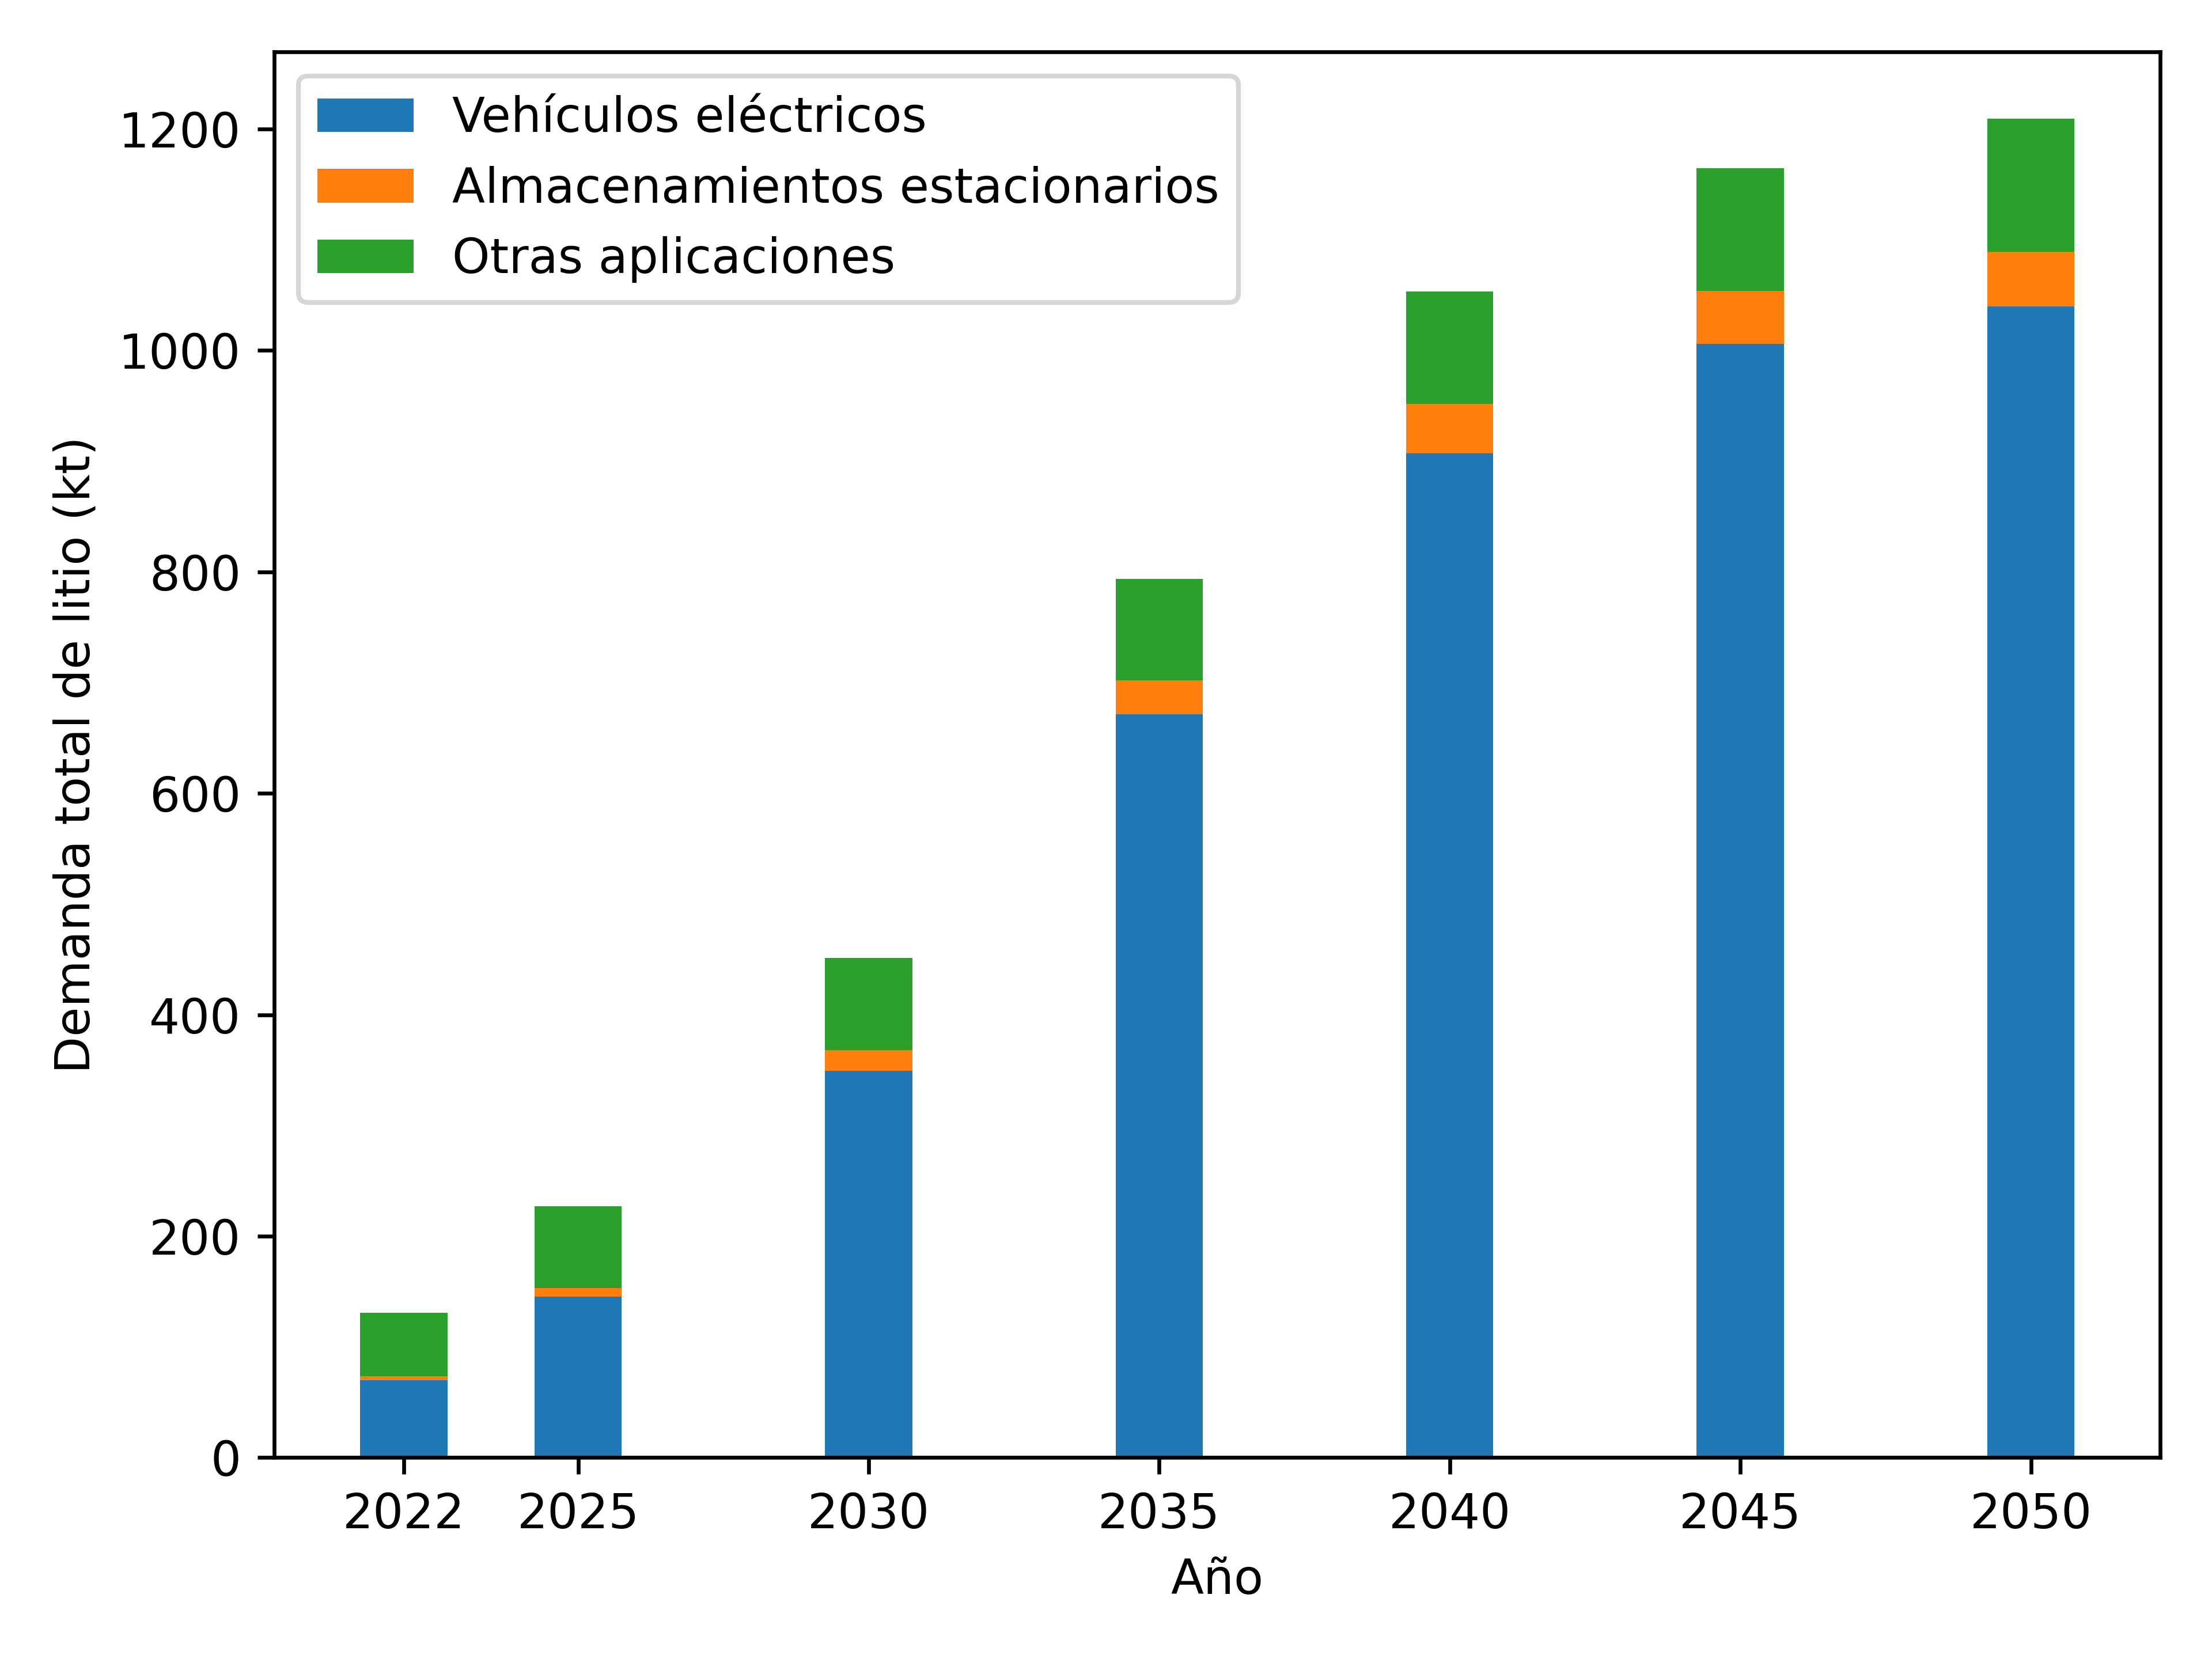
\includegraphics[width=.8\textwidth]{Introduccion/energia/iea-Li.png}
    \caption{Proyección de la demanda total de litio en kilotoneladas para el 
    período 2025-2050 para sus distintas aplicaciones: vehículos eléctricos (en 
    azul), sistemas de almacenamiento de energía estacionarios (en naranja) y
    otras aplicaciones (en verde). Fuente: \cite{IEA}.}
    \label{fig:iea-Li}
\end{figure}
